\section{Sobre los Drones en Ingeniería y Sistemas de Información Geográfica}

  Son dispositivos aéreos que mediante un sensor o cámara pueden capturar luz en direferentes longitudes de onda lo que permite obtener información sobre la superficie terrestre, como por ejemplo: la vegetación, el agua, el suelo, entre otros. Con el uso del efecto de paralaje inicluso, se pueden generar modelos digitales de elevación (DEM). 

  Dentro de los productos que se pueden obtener con el uso de drones, tenemos:
  \begin{itemize}
    \item Mapas topográficos base
    \item Modelos digitales de elevación (DEM)
    \item Ortofotos
    \item Mapas de uso de suelo
    \item Mapas de cobertura vegetal
    \item Mapas de humedad del suelo
    \item Análisis de uso de suelo
    \item Análisis de la calidad del agua
    \item Análisis de la calidad de la cobertura vegetal
  \end{itemize}

  \subsection{RTK}

  RTK (Real-Time Kinematic) es una técnica de posicionamiento que utiliza señales de satélites para determinar la posición de un receptor con una precisión centimétrica. Esta técnica se basa en la comparación de las señales recibidas por el receptor con las señales de referencia enviadas por una estación base, lo que permite corregir los errores causados por la atmósfera y otros factores.

  \subsection{Dron para Topografía:}

  \subsubsection{DJI Mavic 3 Enterprise RTK}

  Es un drone de alta precisión que cuenta con un sistema de posicionamiento RTK (Real-Time Kinematic) que permite obtener datos geoespaciales con una precisión centimétrica. Este drone es ideal para aplicaciones de topografía, cartografía y mapeo, ya que puede capturar imágenes aéreas de alta resolución y generar modelos digitales de elevación (DEM) y ortofotos.

  \begin{figure}[H]
    \centering
    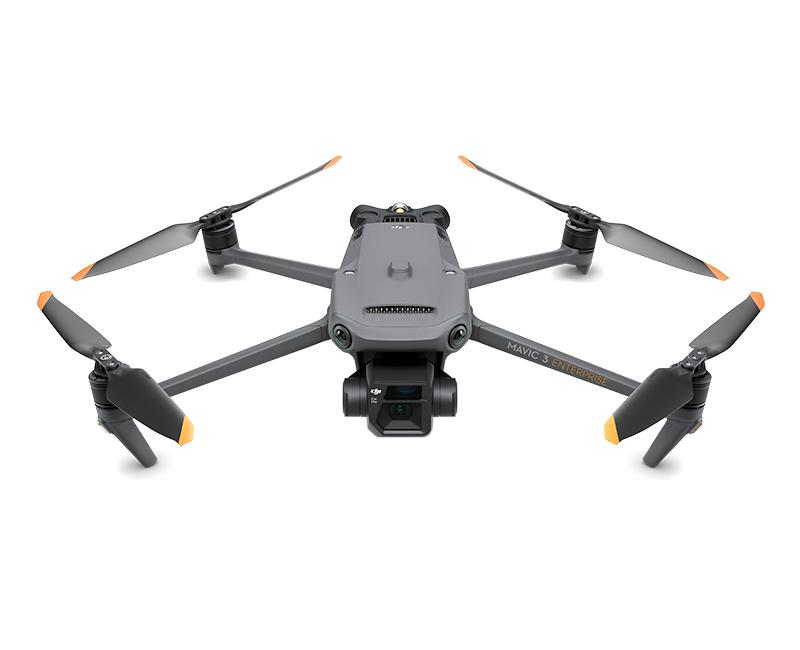
\includegraphics[width=0.5\textwidth]{./assets/DJIRTK.jpg}
     \caption{DJI Mavic 3 Enterprise RTK}
  \end{figure}

  \subsubsection{Características del DJI Mavic 3 Enterprise RTK}

  Características más destacadas de este dron:
  \begin{itemize}
    \item Compacto y portátil
    \item Tiempo máximo de vuelo de 45 minutos
    \item Cámara ancha 4/3 CMOS
    \item Zoom híbrido 56×
    \item Transmisión empresarial DJI O3
    \item Posicionamiento a nivel centimétrico con RTK
    \item Altavoz de alto volumen
  \end{itemize}

  \textbf{Precio: }

  \begin{itemize}
    \item Solo dron * RTK: $5,500 - 6,500$ USD Aproximadamente
  \end{itemize}

  Más información: \url{https://enterprise.dji.com/mavic-3-enterprise}

  \newpage

  \subsection{Dron para Teledetección en Agricultura:}

  \subsubsection{DJI Mavic 3 Multiespectral}

  Es un drone diseñado específicamente para aplicaciones de agricultura de precisión y teledetección. Cuenta con una cámara multiespectral que captura imágenes en diferentes longitudes de onda, lo que permite obtener información sobre la salud de los cultivos, la humedad del suelo y otros factores importantes para la gestión agrícola.

  \begin{figure}[H]
    \centering
    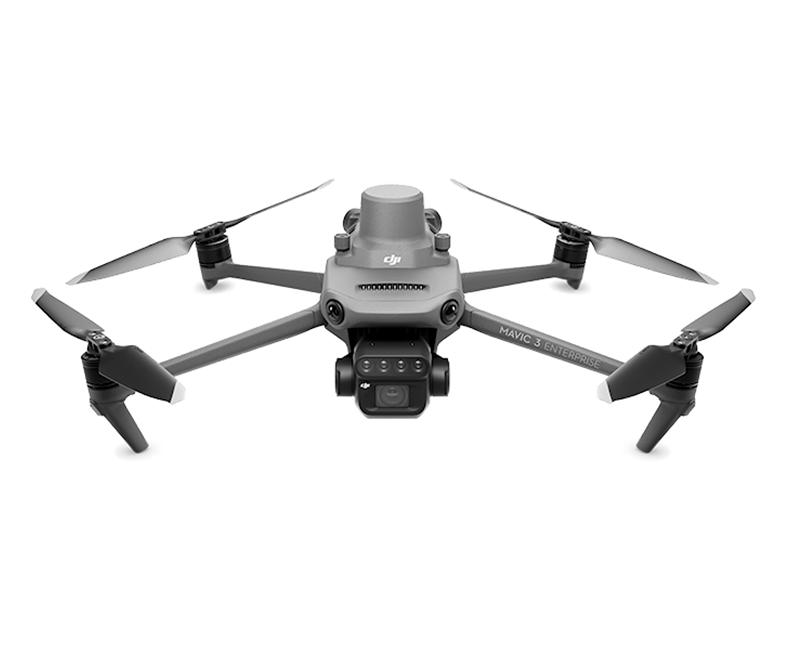
\includegraphics[width=0.5\textwidth]{./assets/DJI_M.jpg}
     \caption{DJI Mavic 3 Multiespectral}
  \end{figure}

  \subsubsection{Características del DJI Mavic 3 Multiespectral}

  Características más destacadas de este dron:
  \begin{itemize}
    \item Compacto y portátil
      \item Tiempo máximo de vuelo de 45 minutos
      \item Cámara ancha 4/3 CMOS
      \item Cámara multiespectral 4 × 5MP G/R/NIR
      \item Transmisión empresarial DJI O3
      \item Posicionamiento a nivel centimétrico con RTK
      \item Altavoz de alto volumen
  \end{itemize}

  \textbf{Precio: }

  \begin{itemize}
    \item Solo dron: $20,000$ PEN Aproximadamente
  \end{itemize}

  Más información: \url{https://dji.pe/mavic-3-multispectral}

  \newpage

  \subsection{Dron para monitoreo de Calidad del Agua:}

  \subsubsection{Matrice 350 RTK + Sensor: MicaSense}

  Es un drone diseñado para aplicaciones de monitoreo ambiental, sirve para todo tipo de aplicaciones, tanto para topografía, agricultura y para monitoreo de la calidad del agua se complementa con el sensor MicaSense que permite capturar imágenes multiespectrales para analizar la calidad del agua, la salud de los ecosistemas acuáticos y otros factores relacionados con el medio ambiente.

  \begin{figure}[H]
    \centering
    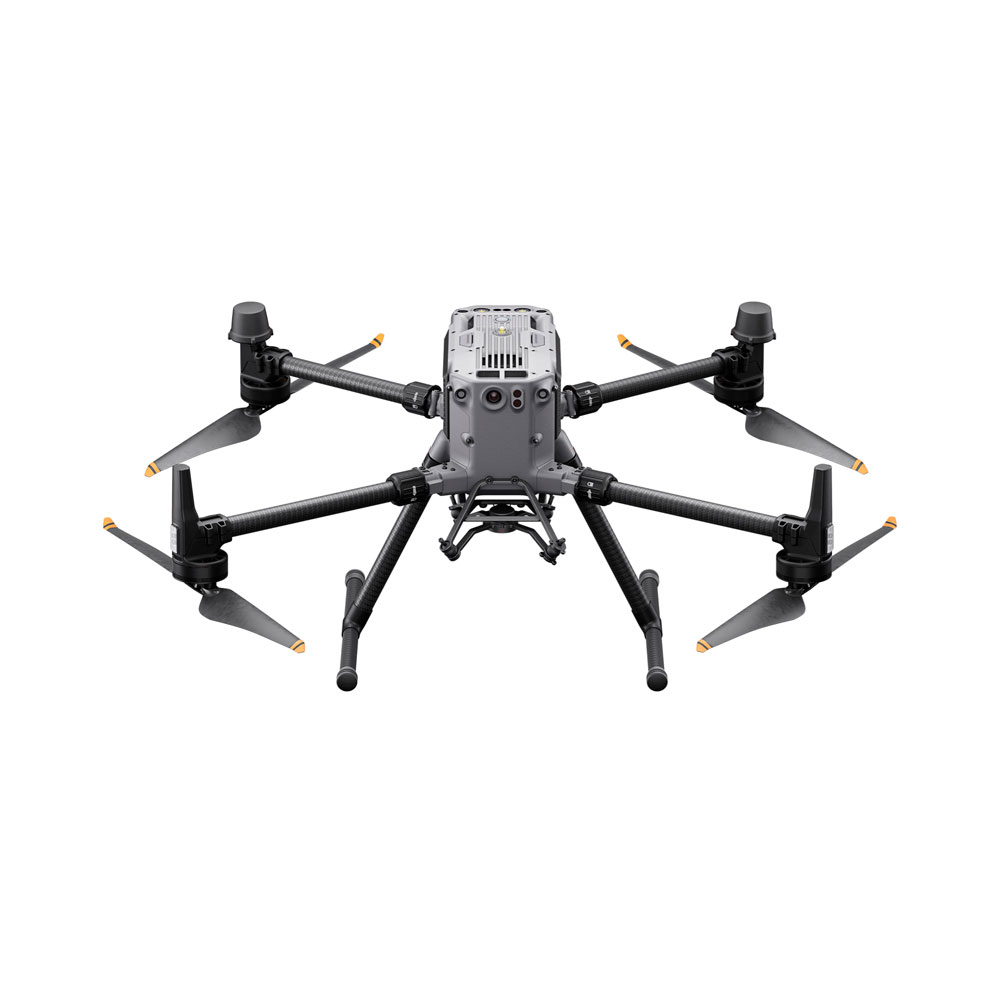
\includegraphics[width=0.5\textwidth]{./assets/matrice.jpg}
     \caption{Matrice 350 RTK + Sensor: MicaSense}
  \end{figure}

  \begin{figure}[H]
    \centering
    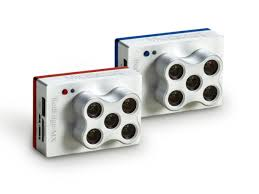
\includegraphics[width=0.5\textwidth]{./assets/mica.jpeg}
     \caption{Sensor: MicaSense}
  \end{figure}

  \newpage


  \subsubsection{Características del Matrice 350 RTK + Sensor: MicaSense}

  Características más destacadas de este dron:
  \begin{itemize}
    \item Tiempo máximo de vuelo de 55 minutos
    \item Clasificación de protección IP55
    \item Peso máximo de carga útil de 2.7 kg
    \item Altitud máxima de vuelo de 7000 m
    \item Resistencia máxima al viento de 12 m/s
    \item Rango de temperatura operativa de -20° a 50° C
  \end{itemize}

  \textbf{Precio: }

  \begin{itemize}
    \item Equipo completo, dron + sensor: $20,000$ USD Aproximadamente
  \end{itemize}

  Más información: \url{https://enterprise.dji.com/matrice-350-rtk}

\newpage
\section{Imágenes Satelitales para el Estudio de la Calidad del Agua}

  Es posible utilizar imágenes satelitales para el estudio de calidad de agua, imágenes que se pueden obtener de manera gratuita y con buena resolución temporal son las de Sentinel-2, esto permite monitorear variables como:

  \begin{itemize}
    \item Clorofila-a
    \item Turbidez
    \item TSS (Total de Sólidos Suspendidos)
    \item Eutrofización
    \item NDWI/MNDWI
    \item Blooms algales
  \end{itemize}

  \textbf{Ejemplo:}

  \begin{figure}[H]
    \centering
    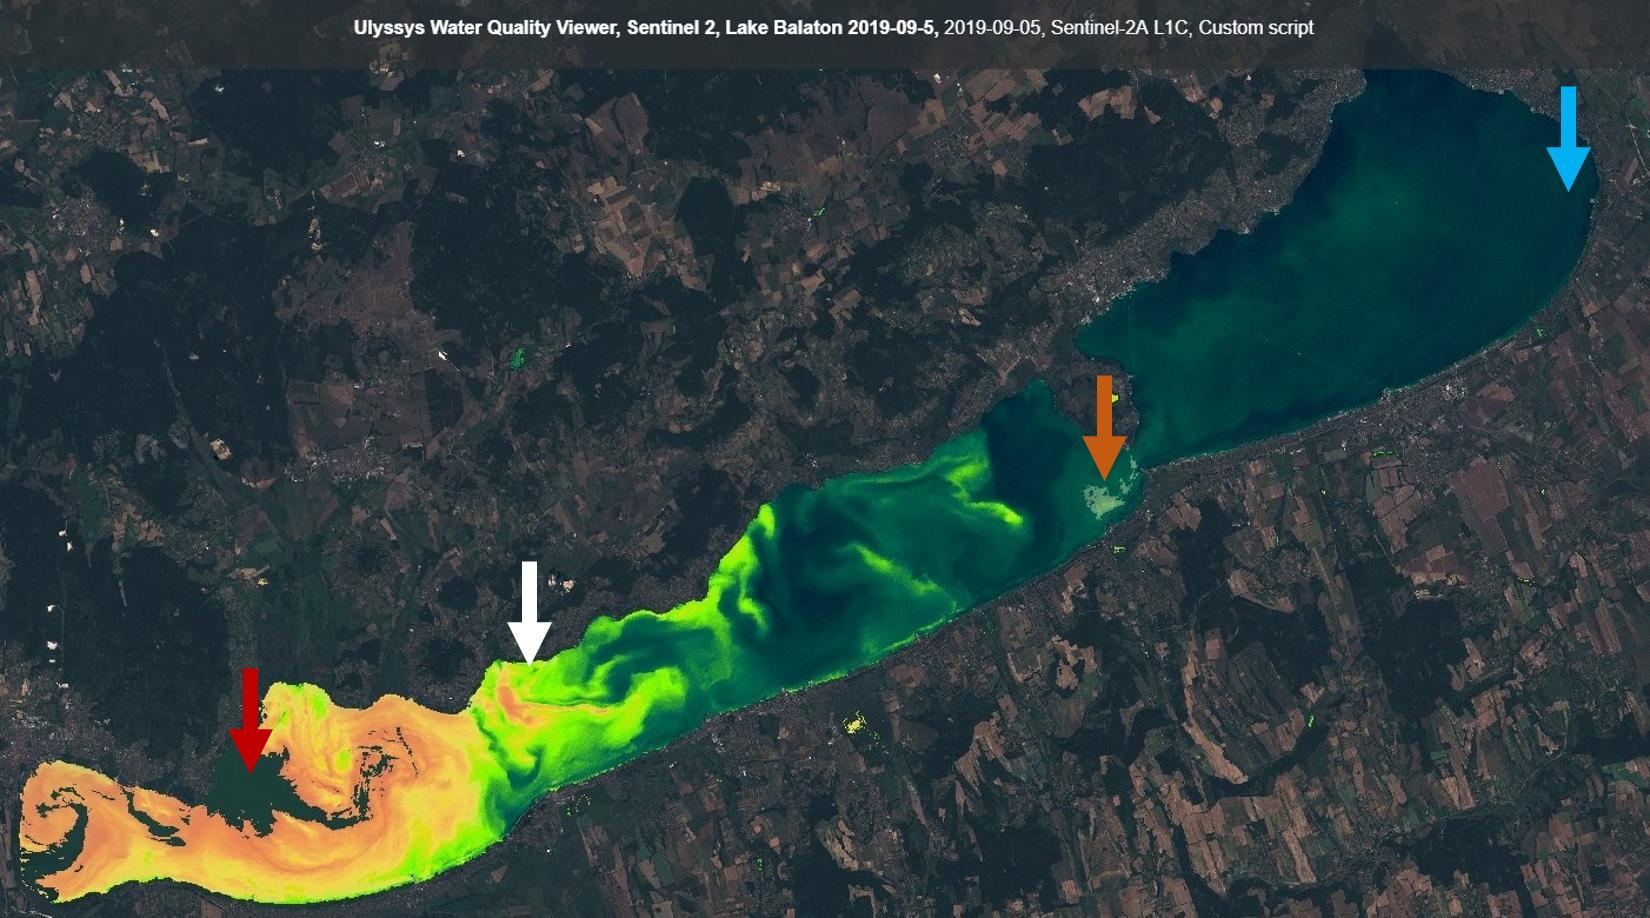
\includegraphics[width=1\textwidth]{./assets/sentinel.jpeg}
     \caption{Ejemplo de imagen satelital Sentinel-2 para el estudio de la calidad del agua}
  \end{figure}